\newpage
\null
\vspace{0.15cm}

\begin{center}
    \Huge{\textbf{\underline{Chapter 5: Deadlock}}}
\end{center}

\vspace{0.25cm}

\setcounter{section}{0}

\section{Processes \& Resources}
\begin{prettyBox}{S}{myblue}
Processes in an \textbf{(OS)} use various resources such as peripherals, variables, and files, following these steps:
\begin{enumerate}
    \item Request a resource, if it is unavailable the process is put on wait.
    \item Hold and use the resource.
    \item Release the resource once the operation is completed.
\end{enumerate}
\end{prettyBox}

\vspace{0.25cm}

\section{Deadlock}
\begin{prettyBox}{What is Deadlock?}{myblue}
Deadlock is a situation where a set of processes becomes blocked because each process is holding a resource and waiting for another resource held by another process to be released.
\end{prettyBox}

\vspace{0.15cm}

\section{Resource-Process Graph}
\begin{center}
    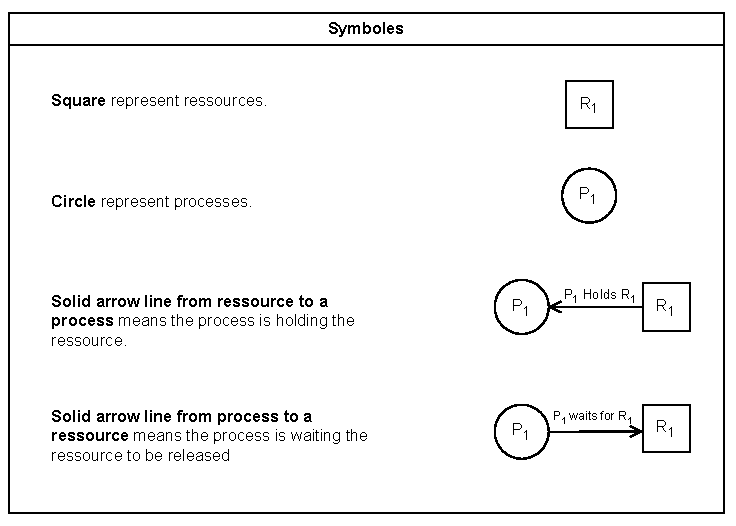
\includegraphics{Chapters/Diagram/Deadlock/sym.drawio.pdf}
\end{center}

\vspace{0.25cm}
\null
\section{Conditions for Deadlock}
\begin{prettyBox}{Coffman Conditions}{myblue}
Deadlock can arise if all the following conditions are met:
\begin{itemize}
    \item \textbf{Mutual Exclusion}: Only one process can hold a resource at a time.
    \item \textbf{Hold and Wait}: A process holding at least one resource is waiting for additional resources held by other processes.
    \item \textbf{No Preemption}: The \textbf{OS} cannot forcibly remove a resource from a process.
    \item \textbf{Circular Wait}: There is a cycle in the graph of two or more processes waiting for each other to release ressources.
\end{itemize}
\end{prettyBox}

\vspace{1cm}

\begin{center}
    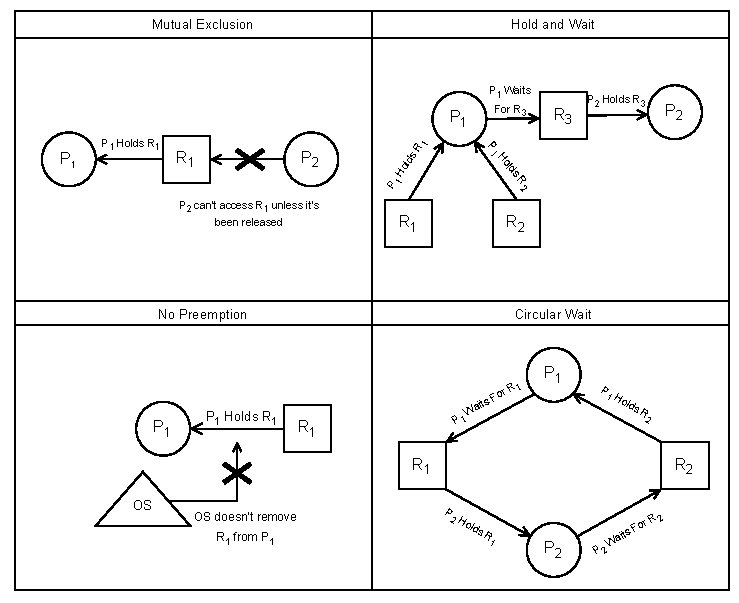
\includegraphics{Chapters/Diagram/Deadlock/coffman.drawio.pdf}
\end{center}

\newpage
\null
\section{Handling Deadlocks}
\begin{prettyBox}{Methods}{myblue}
\begin{itemize}
    \item \textbf{Ignore the Problem}: If resolving deadlocks is too costly, the \textbf{OS} may adopt a laissez-faire approach, ignoring deadlocks and requiring a system reboot if necessary.
    \item \textbf{Detection and Resolution}: The system detects deadlocks, often using algorithms like \textbf{DFS} on the resource allocation graph, and resolves them through one of the following strategies:
    \begin{itemize}
        \item \textbf{Preemption}: Reassign a resource from one process to another, which may lead to issues like inconsistency or lost progress.
        \item \textbf{Rollback}: Restore the system to a previously saved state and reallocate resources to avoid deadlock.
        \item \textbf{Termination}: Kill one or more processes involved in the deadlock to free resources.
    \end{itemize}
    
   \item \textbf{Avoidance}: Dynamically allocate resources in a way that avoids unsafe states, using the \textbf{Banker's Algorithm} to check the safety of each potential allocation before it is made.

    \item \textbf{Prevention}: Prevent deadlocks by ensuring at least one of Coffman’s conditions cannot occur:
    \begin{itemize}
        
\item \textbf{Mutual Exclusion}: Use serialized access (e.g., queues) to eliminate contention by ensuring resources are accessed in an orderly fashion. This doesn't remove mutual exclusion, but it allows the system to control priority, avoiding chaotic competition between processes.
        \item \textbf{Hold and Wait}: Require processes to request all the resources they need at the beginning. 
        While this prevents deadlocks, it can lead to inefficiency because resources may remain idle, and a resource may need to be released to be used by another.
        \item \textbf{No Preemption}: Allow preemption for certain resources by forcibly reallocating them. This
            approach is rarely practical due to the complexity of saving and restoring resource states.
        \item \textbf{Circular Wait}: Resources are assigned increasing numerical labels. Processes must request 
    resources in increasing order of their labels. This ensures that no cycles can form in the resource allocation graph preventing deadlock.
    \end{itemize}
\end{itemize}
\end{prettyBox}

\vspace{0.5cm}
\section{Depth First Search(DFS)}


\begin{prettyBox}{DFS for Deadlock Detection}{myblue}
    To detect a deadlock in the resource-process graph, we use a \textbf{stack} and a \textbf{visited list}. The algorithm proceeds as follows:

\begin{itemize}
    \item Start from any node and push it onto the stack.
    \item Traverse through the graph by exploring neighbors of the current node.
    \item For each node, mark it as visited and push it onto the stack.
\item If a node is encountered that is already in the stack, a \textbf{deadlock} exists, indicating a cycle in the graph.
\item If a node has no unvisited neighbors (i.e., no outgoing edges), \textbf{backtrack} by popping nodes from the stack and continue exploring other unvisited nodes.
    \item Repeat the process until all reachable nodes are visited.
    \item If no cycles are found and all nodes have been explored, \textbf{no deadlock} exists.
\end{itemize}
\end{prettyBox}

\vspace{0.5cm}
\begin{figure}[h!]
    \begin{minipage}{0.6\textwidth}
        \subsubsection*{\underline{Example}}
        Is there a deadlock and if yes what are the processes responsible for them.
        \begin{itemize}
            \item Process \(P_1\) holds \(R_1\) and requests \(R_2\).
            \item Process \(P_2\) holds no resource but requests \(R_3\).
            \item Process \(P_3\) holds no resource but requests \(R_2\).
            \item Process \(P_4\) holds \(R_4\) and requests \(R_2\), \(R_3\).
            \item Process \(P_5\) holds \(R_3\) and requests \(R_5\).
            \item Process \(P_6\) holds \(R_6\) and requests \(R_2\).
            \item Process \(P_7\) holds \(R_5\) and requests \(R_4\).
        \end{itemize}
    \end{minipage}%
    \begin{minipage}{0.4\textwidth}
        \centering
        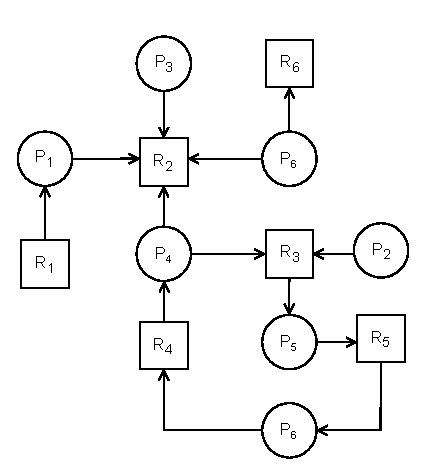
\includegraphics[width=\linewidth]{Chapters/DFS/ex1.1.drawio.pdf}
    \end{minipage}
\end{figure}

\vspace{1.5cm}
\begin{center}
We take \(P_4\) as the starting node 
\end{center}

\begin{center}
    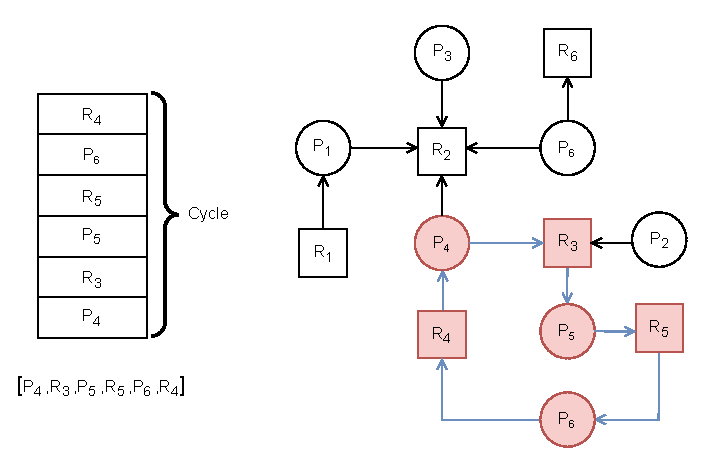
\includegraphics[width=0.7\textwidth]{Chapters/DFS/ex1.2.drawio.pdf}
\end{center}

\vspace{0.25cm}
\begin{center}
 We can notice a cycle in the graph \((P_4,R_3,P_5,R_5,P_6,R_4)\) therefore
There is a deadlock and the processes involved are \(P_4,P_5,P_6\)  
\end{center}

\vspace{1.5cm}
\begin{center}
    \subsubsection*{\underline{\Large{The Cycle}}}
\end{center}

\begin{center}
    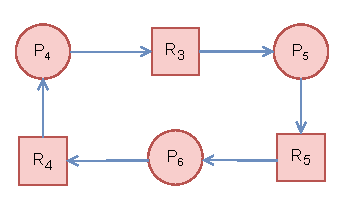
\includegraphics[width=0.4\textwidth]{Chapters/DFS/cycle.pdf}
\end{center}


\section{Banker's Algorithm}

\begin{prettyBox}{Matrix \& Vector Definitions}{myblue}
The following matrices and vectors are used in the Banker's Algorithm:
\begin{itemize}
    \item \textbf{Max}: A matrix indicating the maximum resources each process can request.
    \item \textbf{C}: A matrix representing the currently allocated resources for all processes.
    \item \textbf{Need}: A matrix showing the remaining resources each process requires, calculated as \(Need = Max - C\).
    \item \textbf{A}: A vector of available resources at the start of the algorithm.
    \item \textbf{V}: A vector of available resources at the end of the algorithm.
\end{itemize}
\end{prettyBox}

\vspace{0.25cm}

\begin{prettyBox}{Algorithm Steps}{myblue}
To determine whether the allocation is safe:
\begin{enumerate}
    \item \textbf{Calculate the Need Matrix:} 
        \[
        Need = Max - C
        \]
    \item \textbf{Check Resource Availability:}
    \begin{itemize}
        \item For each process \(i\), check if \(Need(i,:) \leq A\) (i.e., the process’s resource needs are less than or equal to the currently available resources).
        \item If \(Need(i,:) \leq A\), mark the process as completed:
        \begin{itemize}
            \item Set all values in \(Need(i,:)\) to \(0\).
            \item Update \(A\) to reflect the newly available resources:
            \[
            A = A + C(i,:)
            \]
        \end{itemize}
        \item If \(Need(i,:) > A\), move to the next process and repeat the check.
    \end{itemize}
    \item \textbf{Determine Outcome:}
    \begin{itemize}
        \item If all processes are marked , the allocation is safe and the safe sequence is the order of the marked processes.
        \item If some processes remain unmarked and no further \(Need(i,:) \leq A\) condition can be satisfied, a deadlock exists.
    \end{itemize}
\end{enumerate}
\end{prettyBox}

\vspace{0.25cm}

\begin{prettyBox}{Note}{red}
At the end of the algorithm, if the allocation is safe, the available vector \(A\) must equal the final vector \(V\), which can be calculated as:
\[
V_i = A_i + \sum C(:,i)
\]
Thus, for safe allocation:
\[
A = V
\]
\end{prettyBox}

\vspace{0.25cm}

\begin{prettyBox}{Notation}{red}
\begin{itemize}
    \item \(A(i,:)\): All elements of row \(i\) in \(A\).
    \item \(A(:,i)\): All elements of column \(i\) in \(A\).
\end{itemize}
\end{prettyBox}

\vspace{0.5cm}
\subsubsection*{\underline{Example}}

\vspace{0.1cm}
\begin{enumerate}
    \item Calculate Vector V 
    \item Calculate Matrix Need
    \item Is it safe allocation ? if yes give the safe sequence.
\end{enumerate}

\vspace{0.15cm}
\begin{center}
    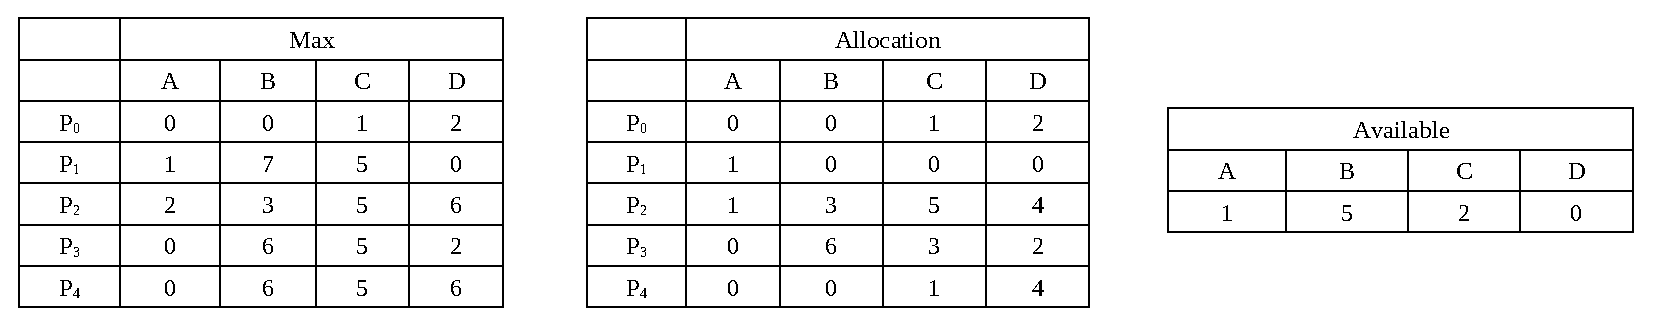
\includegraphics[width=\textwidth]{Chapters/Bank/bank.pdf}
\end{center}

\vspace{0.5cm}
\[\text{Max} = \left[\begin{matrix} 0 & 0 & 1 & 2 \\
                             1 & 7 & 5 & 0\\
                             2 & 3 & 5 & 6\\
                             0 & 6 & 5 & 2\\
                             0 & 6 & 5 & 6\end{matrix}\right]\quad,\quad
    C = \left[\begin{matrix} 0 & 0 & 1 & 2 \\
                             1 & 0 & 0 & 0\\
                             1 & 3 & 5 & 4\\
                             0 & 6 & 3 & 2\\
                             0 & 0 & 1 & 4\end{matrix}\right]\quad,\quad
            A =\left[\begin{matrix} 1 & 5  & 2 & 0   \end{matrix}\right] 
 \]

\vspace{0.75cm}

 \[V_i = A_i + \sum C(:,i)\]

 \vspace{0.15cm}

\[V =\left[\begin{matrix} 0+1+1+0+0+1 & 0+0+3+6+0+5  & 1+0+5+3+1+2  & 2+0+4+2+4+0 \end{matrix}\right] \]

\vspace{0.15cm}

\[V =\left[\begin{matrix} 3 & 14  & 14  & 12 \end{matrix}\right] \]

\vspace{0.75cm}
 \[ \text{Need = Max - C}\quad,\quad\text{Need} = \left[\begin{matrix} 0-0 & 0-0 & 1-1 & 2-2 \\
                             1-1 & 7-0 & 5-0 & 0-0\\
                             2-1 & 3-3 & 5-5 & 6-4\\
                             0-0 & 6-6 & 5-3 & 2-2\\
                     0-0 & 6-0 & 5-1 & 6-4\end{matrix}\right]\quad,\quad
     \text{Need} = \left[\begin{matrix} 0 & 0 & 0 & 0 \\
                             0 & 7 & 5 & 0\\
                             1 & 0 & 0 & 2\\
                             0 & 0 & 2 & 0\\
                     0 & 6 & 4 & 2\end{matrix}\right]\]

\[\text{Need} = \left[\begin{matrix} 0 & 0 & 0 & 0 \\
                             0 & 7 & 5 & 0\\
                             1 & 0 & 0 & 2\\
                             0 & 0 & 2 & 0\\
                     0 & 6 & 4 & 2\end{matrix}\right]\quad,\quad
A =\left[\begin{matrix} 1 & 5  & 2 & 0   \end{matrix}\right] 
\]

\[ \text{Need(1,:)} \leq A \quad \Longrightarrow \quad
\left[\begin{matrix} 0 & 0  & 0 & 0   \end{matrix}\right] \leq
 \left[\begin{matrix} 1 & 5  & 2 & 0   \end{matrix}\right] \]

\[A \gets A + C(1,:)\quad \Longrightarrow \quad A = \left[\begin{matrix} 1+0 & 5+0  & 2+1 & 0+2  \end{matrix}\right] = 
 \left[\begin{matrix} 1 & 5  & 3 & 2  \end{matrix}\right]\]

\vspace{0.5cm}
\[\text{Need} = \left[\begin{matrix} 0 & 0 & 0 & 0 \\
                             0 & 7 & 5 & 0\\
                             1 & 0 & 0 & 2\\
                             0 & 0 & 2 & 0\\
                     0 & 6 & 4 & 2\end{matrix}\right]\quad,\quad
A =\left[\begin{matrix} 1 & 5  & 3 & 2   \end{matrix}\right] 
\]

\[ \text{Need(3,:)} \leq A \quad \Longrightarrow \quad
\left[\begin{matrix} 1 & 0  & 0 & 2   \end{matrix}\right] \leq
 \left[\begin{matrix} 1 & 5  & 3 & 2   \end{matrix}\right] \]

\[A \gets A + C(3,:)\quad \Longrightarrow \quad A = \left[\begin{matrix} 1+1 & 5+3  & 3+5 & 2+4  \end{matrix}\right] = 
 \left[\begin{matrix} 2 & 8  & 8 & 6  \end{matrix}\right]\]

\vspace{0.5cm}
\[\text{Need} = \left[\begin{matrix} 0 & 0 & 0 & 0 \\
                             0 & 7 & 5 & 0\\
                             0 & 0 & 0 & 0\\
                             0 & 0 & 2 & 0\\
                     0 & 6 & 4 & 2\end{matrix}\right]\quad,\quad
A =\left[\begin{matrix} 2 & 8  & 8 & 6   \end{matrix}\right] 
\]

\[ \text{Need(2,:)} \leq A \quad \Longrightarrow \quad
\left[\begin{matrix} 0& 7  & 5 & 0   \end{matrix}\right] \leq
 \left[\begin{matrix} 2 & 8  & 8 & 6   \end{matrix}\right] \]

\[A \gets A + C(2,:)\quad \Longrightarrow \quad A = \left[\begin{matrix} 2+1 & 8+0  & 8+0 & 6+0  \end{matrix}\right] = 
 \left[\begin{matrix} 3 & 8  & 8 & 6  \end{matrix}\right]\]

\vspace{0.5cm}
\[\text{Need} = \left[\begin{matrix} 0 & 0 & 0 & 0 \\
                             0 & 0 & 0 & 0\\
                             0 & 0 & 0 & 0\\
                             0 & 0 & 2 & 0\\
                     0 & 6 & 4 & 2\end{matrix}\right]\quad,\quad
A =\left[\begin{matrix} 3 & 8  & 8 & 6   \end{matrix}\right] 
\]

\[ \text{Need(4,:)} \leq A \quad \Longrightarrow \quad
\left[\begin{matrix} 0& 0  &2 & 0   \end{matrix}\right] \leq
 \left[\begin{matrix} 3 & 8  & 8 & 6   \end{matrix}\right] \]

\[A \gets A + C(4,:)\quad \Longrightarrow \quad A = \left[\begin{matrix} 3+0 & 8+6  & 8+3 & 6+2  \end{matrix}\right] = 
 \left[\begin{matrix} 3 & 14  & 13 & 8  \end{matrix}\right]\]

\newpage
\[\text{Need} = \left[\begin{matrix} 0 & 0 & 0 & 0 \\
                             0 & 0 & 0 & 0\\
                             0 & 0 & 0 & 0\\
                             0 & 0 & 0 & 0\\
                     0 & 6 & 4 & 2\end{matrix}\right]\quad,\quad
A =\left[\begin{matrix} 3 & 14  & 13 & 8   \end{matrix}\right] 
\]

\[ \text{Need(5,:)} \leq A \quad \Longrightarrow \quad
\left[\begin{matrix} 0& 6  &4 & 2   \end{matrix}\right] \leq
 \left[\begin{matrix} 3 & 14  & 13 & 8   \end{matrix}\right] \]

\[A \gets A + C(5,:)\quad \Longrightarrow \quad A = \left[\begin{matrix} 3+0 & 14+0  & 13+1 & 8+4  \end{matrix}\right] = 
 \left[\begin{matrix} 3 & 14  & 14 & 12  \end{matrix}\right]\]

\vspace{0.5cm}
\[\text{Need} = \left[\begin{matrix} 0 & 0 & 0 & 0 \\
                             0 & 0 & 0 & 0\\
                             0 & 0 & 0 & 0\\
                             0 & 0 & 0 & 0\\
                     0 & 0 & 0 & 0\end{matrix}\right]\quad,\quad
A =\left[\begin{matrix} 3 & 14  & 14 & 12   \end{matrix}\right] 
\]

\vspace{0.5cm}
\begin{center}
 All processes have been marked therefore the allocation is safe and the safe sequence is
\(P_0,P_2,P_1,P_3,P_4\)   
\end{center}

\begin{prettyBox}{Note}{red}
There can be many correct safe sequence for the same allocation 
\end{prettyBox}
